
\section{Preliminary}
\subsection{Basics}
{ \setbeamercolor{background canvas}{bg=hl_bg}
  \setbeamercolor{normal text}{fg=hl_fg}
  \setbeamercolor{frametitle}{fg=hl_fg}
  \begin{frame}{A Guide to This Dissertation}
    \usebeamercolor[fg]{normal text}
    \centering
    \begin{tikzpicture}
      \tikzstyle{nnode} = [rectangle, rounded corners=2pt, inner sep = 6pt,  align=center]
      \tikzstyle{rnode} = [draw=black, rectangle, rounded corners=2pt, inner sep = 6pt, align=center]

      \begin{scope}[xshift=-0.5cm]
        \node[rnode, fill=white, text=black] (PandG) at (0,0) {Probability\\ \& \\ Graph};
        \node[rnode, fill=white, text=black] (mrf) at (-2,-2) {Undirected\\
          MRFs};
        \node[rnode, fill=white, text=black] (bn) at (2,-2) {Directed\\
          BNs};
        \begin{scope}[on background layer]
          \node[rnode, inner sep = 12pt, fill=gray, opacity=0.9, fit=(PandG)(mrf)(bn)] (core) {};
          \node[nnode] at (0,-1.5) {Preliminary \\ Chpt. 1, 2};
        \end{scope}
      \end{scope}
      \draw[black,->] (PandG) to (mrf);
      \draw[black,->] (PandG) to (bn);
      
      \node[rnode, fill=white, text=black] (exact) at (0, -4) {Exact Inference \\ (Briefed Chpt. 2)};
      \draw[black,->] (core) to (exact);
      
      \node[rnode, fill=white, text=black] (apprx) at (-4, -4) {Approximate Inference\\
        Chpt. 3, 4};
      \node[rnode, fill=white, text=black] (mrfLearn) at (-5, -2) {Learning\\ Chpt. 5};
      
      \draw[black,->] (mrf) to (apprx);
      \draw[black,->] (mrf) to (mrfLearn);

      \node[rnode, fill=white, text=black] (em) at (4, -4) {Learning \\ (incomplete observation) \\ Chpt. 6};
      \node[rnode, fill=white, text=black] (hmm) at (5, -2) {Temporary\\Model \\ Chpt. 7};
      \node[rnode, fill=white, text=black] (llkFree) at (4.5, 0) {Likelihood-free\\
        (Implicit) \\ Chpt. 8};
      
      \draw[black,->] (bn) to (em);
      \draw[black,->] (bn) to (hmm);
      \draw[black,->] (bn) to (llkFree);
      

      

    \end{tikzpicture}
  \end{frame}
}

\begin{frame}{What are Probabilistic Graphical Models}
  \onslide<1->{
    Informally...
    \begin{itemize}[label={$\bullet$}]
    \item attributes of our interests in a system $\rightarrow$ variable nodes
    \item relationship of these factors $\rightarrow$ structures of a graph
    \end{itemize}
    Intrinsic property: \textbf{reasoning with uncertainty}
  }\\
  \vskip 0.8cm
  \onslide<2->{
    A directed/undirected graph encoding dependencies/indepedencies of distribution $p(\bm{x}; \bm{\theta})$:
    \begin{itemize}[label={$\bullet$}]
    \item A BN/Generative model is a directed graph
      \begin{itemize}[label={$\bullet$}]
      \item $p(\bm{x}; \bm{\theta}) = \prod_{n=1}^{N}p(x_n| \Pp(x_n))$
      \item $\Pp(\cdot)$ are parent nodes
      \item the local functions are proper distributions
      \end{itemize}
      
    \item An MRF denoted by an undirected graph $\Gg(\Vv, \Ee)$
      \begin{itemize}[label=$\bullet$]
      \item The probability distribution (Gibbs distribution) is $p(\bm{x}; \bm{\theta}) = \frac{1}{Z(\bm{\theta})} \prod_{a\in\Ii} \psi_a(\bm{x}_a; \bm{\theta}_a)$
      \item  $a$ indexes potential functions $\Ii=\{\psi_A, \psi_B, \cdots, \psi_M\}$
      \item $Z(\bm{\theta}) = \sum_{\bm{x}}\prod_{a} \psi_a(\bm{x}_a;\bm{\theta}_a)$.
      \end{itemize}
    \end{itemize}
  }
  
\end{frame}
\begin{frame}{Usage of Graphical Models}
  \begin{itemize}[label={$\bullet$}]
  \item The common inference problems:
    \begin{itemize}[label={$\bullet$}]
    \item Computing the likelihood of observed data.
    \item Computing the marginals distribution $p(\bm{x}_A)$ over particular subset $A \subset \Vv$ of nodes
    \item Computing the conditional distribution $p(\bm{x}_A | \bm{x}_{B})$, 
    \item Computing the partition function or the Helmholtz free energy (for MRFs)
    \end{itemize}
  \item Learning:
    \begin{itemize}[label=$\bullet$]
      \item To model or determine $p(\bm{x}; \bm{\theta})$.
      \end{itemize}
  \end{itemize}
  

  \onslide<2->{
    Two key components interacting with each other:
    \begin{figure}[!t]
      \centering
      \begin{tikzpicture}
        \tikzstyle{cnode} = [thick, draw=black, ellipse, inner sep = 2pt,  align=center]
        \tikzstyle{fnode} = [thick, draw=black, ellipse, inner sep = 10pt,  align=center]
        
        \node[cnode] (infn) at (0,0) {Inference};
        \node[cnode] (lern) at (3,0) {Learning};
        
        \node[fnode, fit=(infn)(lern)] (box) {};
        \node[] at (1.4, -0.6) {\textbf{Probabilistic} Graphical Model};
        \draw[->,line width=0.2mm] (infn) to[out=15, in=165] (lern);
        \draw[->,line width=0.2mm] (lern) to[out=195, in=-15] (infn);
      \end{tikzpicture}

    \end{figure}
  }

\end{frame}








%%%%%%%%%%%%%%%%%%%%%%%%%%%%%%%%%%%%%%%%%%%%%%%%%%%%%% 
% ------------------------------------------------
%%%%%%%%%%%%%%%%%%%%%%%%%%%%%%%%%%%%%%%%%%%%%%%%%%%%%% 
% \section{Inference}



\subsection{Intuition of Message Passing}
\begin{frame}{What is the state of $x$?}
  \framesubtitle{A toy example}
  Assume that we are interested into the state of node $i$ in an MRF, it can be answered by
  \begin{itemize}[label={$\bullet$}]
  \item the probability $p(x_i)$, or
  \item an empirical version, a collection of samples $\left\{ x_i^n \right\}_{n=1}^{N}$
  \end{itemize}
  It is similar for the case when $\bm{x}$ is of interests, instead of $x_i$.
  \begin{figure}
    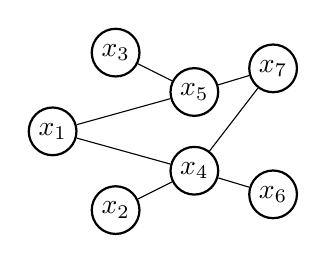
\begin{tikzpicture}
      % \tikzstyle{enode} = [thick, draw=blue, circle, inner sep = 3pt,
      % align=center]
      \tikzstyle{enode} = [thick, draw=black, circle, inner sep = 2pt,  align=center]
      \node[enode] (x1) at (-0.8,0) {$x_1$};
      \node[enode] (x2) at (0,-1) {$x_2$};
      \node[enode] (x3) at (0,1) {$x_3$};
      \node[enode] (x4) at (1,-0.5) {$x_4$};
      \node[enode] (x5) at (1,0.5) {$x_5$};
      \node[enode] (x6) at (2,-0.8) {$x_6$};
      \node[enode] (x7) at (2,+0.8) {$x_7$};

      \draw[-] (x1) to (x4);
      \draw[-] (x1) to (x5);
      \draw[-] (x2) to (x4);
      
      \draw[-] (x3) to (x5);
      \draw[-] (x4) to (x6);
      \draw[-] (x4) to (x7);
      \draw[-] (x5) to (x7);
    \end{tikzpicture}
    \captionsetup{labelformat=empty,justification=centering}
    \caption{what is the state of $x_4$}
    
  \end{figure}
  
\end{frame}

\begin{frame}{What is the state of $x$?}
  \begin{columns}
    \column{0.5\textwidth}
    {Gibbs sampling: let us guess by sampling}
    \vskip 0.5cm
   Sample iteratively: $  x_i \sim p(x_i|\bm{x}_{-i}) \sim p(x_i,\bm{x}_{-i})$
  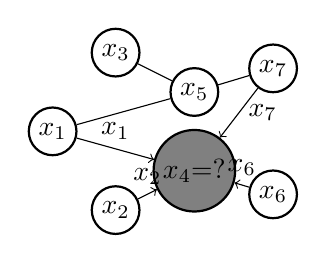
\begin{tikzpicture}
        % \tikzstyle{enode} = [thick, draw=blue, circle, inner sep = 3pt,
        % align=center]
        \tikzstyle{enode} = [thick, draw=black, circle, inner sep = 2pt,  align=center]
        \node[enode] (x1) at (-0.8,0) {$x_1$};
        \node[enode] (x2) at (0,-1) {$x_2$};
        \node[enode] (x3) at (0,1) {$x_3$};
        \node[enode, fill=gray] (x4) at (1,-0.5) {$x_4$=?};
        \node[enode] (x5) at (1,0.5) {$x_5$};
        \node[enode] (x6) at (2,-0.8) {$x_6$};
        \node[enode] (x7) at (2,+0.8) {$x_7$};

        \draw[->] (x1) to node[above] {$x_1$} (x4);
        \draw[-] (x1) to (x5);
        \draw[->] (x2) to node[above] {$x_2$} (x4);
        
        \draw[-] (x3) to (x5);
        \draw[->] (x6) to node[above] {$x_6$} (x4);
        \draw[->] (x7) to node[right] {$x_7$} (x4);
        \draw[-] (x5) to (x7);
      \end{tikzpicture}
      \vskip 0.5cm
      Queries by collected samples $\left\{ \bm{x}^n \right\}_{1}^{N}$.
      
    \column{0.5\textwidth}
    Mean Field and BP: \textit{message in form of sample values $\rightarrow$ message in form of belief}
    \vskip 0.5cm
    Propagating beliefs iteratively
      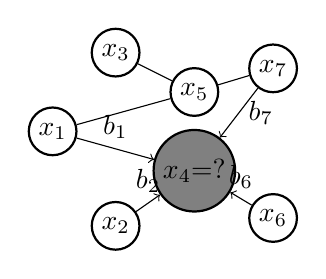
\begin{tikzpicture}
      \tikzstyle{enode} = [thick, draw=black, circle, inner sep = 2pt,  align=center]
      \node[enode] (x1) at (-0.8,0) {$x_1$};
      \node[enode] (x2) at (0,-1.2) {$x_2$};
      \node[enode] (x3) at (0,1) {$x_3$};
      \node[enode, fill=gray] (x4) at (1,-0.5) {$x_4$=?};
      \node[enode] (x5) at (1,0.5) {$x_5$};
      \node[enode] (x6) at (2,-1.1) {$x_6$};
      \node[enode] (x7) at (2,+0.8) {$x_7$};

      \draw[->] (x1) to node[above=0.05mm] {$b_1$} (x4);
      \draw[-] (x1) to (x5);
      \draw[->] (x2) to node[above=0.05mm] {$b_2$}(x4);
      
      \draw[-] (x3) to (x5);
      \draw[->] (x6) to node[above=0.05mm] {$b_6$} (x4);
      \draw[->] (x7) to node[right] {$b_7$} (x4);
      \draw[-] (x5) to (x7);
    \end{tikzpicture}
    \vskip 0.5cm
    Queries by collected samples $\left\{ b_i\right\}$.

    % Corresponding to minimization of \textbf{variational free energy $F_v(b)$  with trial $b$ in fully-factorized form for univariant $\{b_i\}$}.
    \end{columns}
    \let\thefootnote\relax\footnotetext{
      Intuition from \textit{Gibbs (variational) free energy}
        \begin{equation*}
          F_V(b) = \mathrm{KL}(b( \bm{x}) || p(\bm{x}; \bm{\theta})) - \log{Z(\bm{\theta})}
        \end{equation*}
        with trial $b(\bm{x})$. Instance: Bethe free energy.
        }
\end{frame}

% \begin{frame}{What is the state of $x$?}
%   Naive Mean Field: \textbf{message in form of sample values $\rightarrow$ message in form of belief}
%   \begin{figure}
    
%     \begin{tikzpicture}
%       \tikzstyle{enode} = [thick, draw=black, circle, inner sep = 2pt,  align=center]
%       \node[enode] (x1) at (-0.8,0) {$x_1$};
%       \node[enode] (x2) at (0,-1.2) {$x_2$};
%       \node[enode] (x3) at (0,1) {$x_3$};
%       \node[enode, fill=gray] (x4) at (1,-0.5) {$x_4$=?};
%       \node[enode] (x5) at (1,0.5) {$x_5$};
%       \node[enode] (x6) at (2,-1.1) {$x_6$};
%       \node[enode] (x7) at (2,+0.8) {$x_7$};

%       \draw[->] (x1) to node[above=0.05mm] {$b_1$} (x4);
%       \draw[-] (x1) to (x5);
%       \draw[->] (x2) to node[above=0.05mm] {$b_2$}(x4);
      
%       \draw[-] (x3) to (x5);
%       \draw[->] (x6) to node[above=0.05mm] {$b_6$} (x4);
%       \draw[->] (x7) to node[right] {$b_7$} (x4);
%       \draw[-] (x5) to (x7);
%     \end{tikzpicture}
%   \end{figure}
%   Corresponding to minimization of \textbf{variational free energy $F_v(b)$  with trial $b$ in fully-factorized form for univariant $\{b_i\}$}.
%   \let\thefootnote\relax\footnotetext{\tiny
%     Iterative sampling $\rightarrow$ iterative belief update via  
%     \begin{equation*}
%       \log{b_i(x_i)} \propto \sum_{a \in \mathrm{ne}_i} \sum_{\bm{x}_{a} \backslash x_i} \prod_{j\in {a}\backslash i} b_j(x_j)\log{\phi_{a}}(\bm{x}_{a};\bm{\theta}_{a}).
%     \end{equation*}  
%   }
% \end{frame}

% \begin{frame}{What is the state of $x$?}
%   \framesubtitle{Belief propagation (BP): let us guess by propagating belief}
%   \onslide<1->{

%     Proposed by Pearl (1982) for Bayesian networks (tree-structured graphs), which then widely used for general graphs (loopy BP).
    
%     {Yedidia, et al, connected the loopy BP with stationary points of \textbf{Bethe free energy}
%       \begin{align*}
%         F_{Bethe}(b) = \sum_{a\in \Ff} \sum_{\bm{x}_{a}}
%         b_{a}(\bm{x}_{a})\log{\frac{b_{a}(\bm{x}_{a})}{\phi_{a}(\bm{x}_{a})}
%         } -  \sum_{i=1}^{N} (|\mathrm{ne}_i| - 1) \sum_{x_i} b_i(x_i) \log{b_i(x_i)},
%       \end{align*}
%     }
    
%     Corresponding to minimization of approximated \textbf{variational free energy $F_v(b)$  with trial $b$ includes $\{b_i\}$ and $\{b_a\}$}.

%   }
%   \let\thefootnote\relax\footnotetext{\tiny
%     \vskip -0.8cm
%     \begin{align*}
%       \mathrm{msg: factor~ to~ variable} ~~ m_{a\rightarrow i}(x_i) & \propto \sum_{\bm{x}_{a} \backslash x_i}
%                                                                       \phi_{a}(\bm{x}_{a}) \prod_{j \in a \backslash i} m_{j\rightarrow a}(x_j), \\
%       \mathrm{msg: variable~ to~ factor} ~~  m_{j\rightarrow a}(x_j) & \propto  \prod_{a^{\prime} \in \mathrm{ne}_j
%                                                                        \backslash a} m_{a^{\prime}\rightarrow j}(x_j)
%     \end{align*}
%     See, D. Liu, M. T. Vu, Z. Li, and Lars K. Rasmussen. $\alpha$ belief propagation for approximate inference. 2020 \\
%     D. Liu, N. N. Moghadam, L. K. Rasmussen, etc. $\alpha$ belief propagation as fully factorized approximation. In
%     GlobalSIP, 2019.
%     for alternative view to loopy BP.
%   }
  
% \end{frame}



% { \setbeamercolor{background canvas}{bg=hl_bg}
%   \setbeamercolor{normal text}{fg=hl_fg}
%   \setbeamercolor{frametitle}{fg=hl_fg}
%   \begin{frame}
%     \usebeamercolor[fg]{normal text}
%     \begin{center}
%       {\large
%         Play with
%         \textbf{Gibbs (variational) free energy}
%         \begin{equation*}
%           F_V(b) = \mathrm{KL}(b( \bm{x}) || p(\bm{x}; \bm{\theta})) - \log{Z(\bm{\theta})}
%         \end{equation*}
%         with trial $b(\bm{x})$.
%       }
%     \end{center}
    
%   \end{frame}
% }


%%% Local Variables:
%%% mode: latex
%%% TeX-master: "../ppgm_slide"
%%% End:
